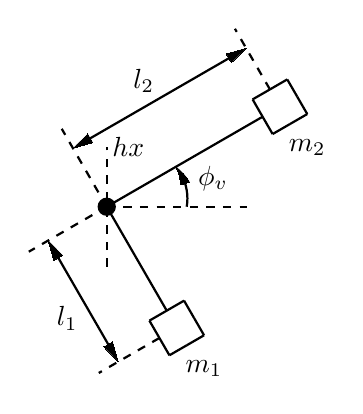
\begin{tikzpicture}[scale=2.54]
% dpic version 2015.10.28 option -g for TikZ and PGF 1.01
\ifx\dpiclw\undefined\newdimen\dpiclw\fi
\global\def\dpicdraw{\draw[line width=\dpiclw]}
\global\def\dpicstop{;}
\dpiclw=0.8bp
\dpicdraw[fill=black](0,0) circle (0.015748in)\dpicstop
\dpicdraw (0.779426,0.449983)
 --(0.829429,0.363382)\dpicstop
\dpicdraw (0.829429,0.363382)
 --(0.916032,0.413381)\dpicstop
\dpicdraw (0.916032,0.413381)
 --(1.002636,0.46338)\dpicstop
\dpicdraw (1.002636,0.46338)
 --(0.952641,0.549985)\dpicstop
\dpicdraw (0.952641,0.549985)
 --(0.902646,0.636591)\dpicstop
\dpicdraw (0.902646,0.636591)
 --(0.816038,0.5866)\dpicstop
\dpicdraw (0.816038,0.5866)
 --(0.729431,0.53661)\dpicstop
\dpicdraw (0.729431,0.53661)
 --(0.779433,0.450009)\dpicstop
\dpicdraw (0.779426,0.449983)
 --(0,0)\dpicstop
\draw (1.002636,0.363382) node[below=-1.5bp]{$m_2$};
\dpicdraw (0.263412,-0.65621)
 --(0.313415,-0.742811)\dpicstop
\dpicdraw (0.313415,-0.742811)
 --(0.400018,-0.692813)\dpicstop
\dpicdraw (0.400018,-0.692813)
 --(0.486621,-0.642814)\dpicstop
\dpicdraw (0.486621,-0.642814)
 --(0.436627,-0.556208)\dpicstop
\dpicdraw (0.436627,-0.556208)
 --(0.386632,-0.469603)\dpicstop
\dpicdraw (0.386632,-0.469603)
 --(0.300024,-0.519593)\dpicstop
\dpicdraw (0.300024,-0.519593)
 --(0.213416,-0.569584)\dpicstop
\dpicdraw (0.213416,-0.569584)
 --(0.263419,-0.656185)\dpicstop
\dpicdraw (0.300024,-0.519593)
 --(0,0)\dpicstop
\draw (0.486621,-0.742811) node[below=-1.5bp]{$m_1$};
\dpicdraw[dashed](0.816038,0.5866)
 --(0.641057,0.889712)\dpicstop
\dpicdraw[dashed](0,0)
 --(-0.224976,0.389725)\dpicstop
\filldraw[line width=0bp](0.623198,0.720631)
 --(0.697301,0.792281)
 --(0.598198,0.763933) --cycle\dpicstop
\filldraw[line width=0bp](-0.094628,0.363943)
 --(-0.168732,0.292294)
 --(-0.069629,0.320642) --cycle\dpicstop
\dpicdraw (0.677464,0.780828)
 --(-0.148894,0.303747)\dpicstop
\draw (0.264285,0.542287) node[above left=-1.5bp]{$l_2$};
\dpicdraw[dashed](0.263412,-0.65621)
 --(-0.039696,-0.831201)\dpicstop
\dpicdraw[dashed](0,0)
 --(-0.389715,-0.224994)\dpicstop
\filldraw[line width=0bp](-0.01392,-0.700852)
 --(0.057733,-0.774952)
 --(0.02938,-0.675851) --cycle\dpicstop
\filldraw[line width=0bp](-0.220633,-0.242846)
 --(-0.292286,-0.168745)
 --(-0.263934,-0.267847) --cycle\dpicstop
\dpicdraw (0.046279,-0.755116)
 --(-0.280832,-0.188582)\dpicstop
\draw (-0.117277,-0.471849) node[below left=-1.5bp]{$l_1$};
\dpicdraw[dashed](0,0)
 --(0.7,0)\dpicstop
\filldraw[line width=0bp](0.392269,0.116546)
 --(0.370058,0.109531)
 ..controls (0.367936,0.140904) and (0.359914,0.171595)
 ..(0.346413,0.199995)
 ..controls (0.374131,0.179484) and (0.397306,0.15346)
 ..(0.414481,0.123561)
 --(0.392269,0.116546)\dpicstop
\dpicdraw[line width=0.8bp](0.372011,0.162387)
 ..controls (0.399424,0.112977) and (0.40929,0.055737)
 ..(0.4,-0)\dpicstop
\draw (0.53126,0.142346) node{$\phi_v$};
\dpicdraw[dashed](0,-0.3)
 --(0,0.3)\dpicstop
\draw (0,0.3) node[right=-1.5bp]{$hx$};
\end{tikzpicture}
